\documentclass[12pt]{article}
\usepackage[english]{babel}
\usepackage[utf8x]{inputenc}
\usepackage[T1]{fontenc}
\usepackage{listings}
\usepackage{bookmark}
\usepackage{tikz}
\usepackage{/Users/songye03/Desktop/math_tex/style/quiver}
\usepackage{/Users/songye03/Desktop/math_tex/style/scribe}
\usepackage{fancyhdr}

\begin{document}


\lhead{Songyu Ye}
\rhead{\today}
\cfoot{\thepage}

\title{Conormal varieties}

\author{Songyu Ye}
\date{\today}
\maketitle


\begin{abstract}
	Spoke with Allen today about conormal varieties.
\end{abstract}

\tableofcontents

\section{Introduction}
We are interested in the $B_- \times B_+$ orbits in $M_{m,n}$.
These are Matrix Schubert Varieties formed by looking at
Northeast rank conditions, Fulton's essential set.

\vspace{1em}
We are interested in the conormal variety to the $B_- \times B_+$ orbit
through the partial permutation matrix $\pi$. This variety \begin{align*}
	C(B_- \pi B_+) \subset M_{m,n} \times M_{m,n}^*
\end{align*} satisfies the following equations (and more but they
are not important for now) \begin{align*}
	p_1(C(B_- \pi B_+)) \text{ satisfies NE rank conditions for } \pi \\
	p_2(C(B_- \pi B_+)) \text{ satisfies SW rank conditions for } \pi^*
\end{align*} where $p_1, p_2$ are the projections to the first and second
factors, and $\pi^*$ is defined combintorially as the partial permutation shown
in red.

\begin{center}
	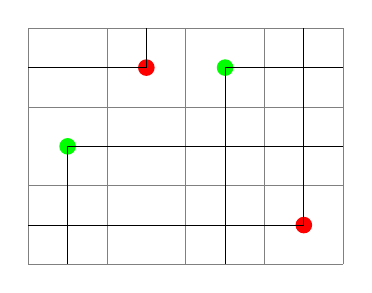
\begin{tikzpicture}
		\draw[step=1cm,gray,very thin] (0,0) grid (4,3);
		\foreach \x in {1,2,3,4} {
				\foreach \y in {1,2,3} {
						\node at (\x-0.5,3.5-\y) {};
					}
			}

		\fill[red] (1.5,2.5) circle (3pt); % (1,2)
		\fill[green] (0.5,1.5) circle (3pt); % (2,1)
		\fill[green] (2.5,2.5) circle (3pt); % (1,3)
		\fill[red] (3.5,0.5) circle (3pt); % (3,4)

		% Draw lines for green dots
		\draw[black] (0.5,1.5) -- (4,1.5); % East line from (2,1)
		\draw[black] (0.5,1.5) -- (0.5,0); % South line from (2,1)
		\draw[black] (2.5,2.5) -- (4,2.5); % East line from (1,3)
		\draw[black] (2.5,2.5) -- (2.5,0); % South line from (1,3)

		% Draw lines for red dots
		\draw[black] (1.5,2.5) -- (1.5,3); % North line from (1,2)
		\draw[black] (1.5,2.5) -- (0,2.5); % West line from (1,2)
		\draw[black] (3.5,0.5) -- (3.5,3); % North line from (3,4)
		\draw[black] (3.5,0.5) -- (0,0.5); % West line from (3,4)

	\end{tikzpicture}
\end{center}

The resulting equations cut out the conormal variety
and some other stuff of codimension 2 or more. Therefore, these equations are
sufficient to know when components of the conormal variety to the stratification
are smooth.

\vspace{1em}
Let $\Lambda\subset T^*M_{m,n}$ be the conormal variety to the Matrix Schubert
Variety stratification. This means that we are considering the union \begin{align*}
	\Lambda = \bigcup_{\pi} C(B_- \pi B_+)
\end{align*}
There is the theorem that when $G$ acts on $M$, then $G$ acts on $T^*M$ Hamiltonianly and
there is a moment map
$\mu: M \to \mathfrak{g}^*$ such that \begin{align*}
	\Phi^{-1}(0) = \Lambda = \bigcup C(\text{orbits in $M$})
\end{align*}

In our situation, we have the moment map for the action of $B_{-}\times B_{+} \hookrightarrow G\times G$
acting on $M_{m,n}$. We have the composition \begin{align*}
    (X,Y) \mapsto (XY^T,-Y^TX) \mapsto (\text{Lower}(XY^T), \text{Upper}(-Y^TX))
\end{align*} where I want the lower triangular
part of the first matrix and the upper triangular part of the second matrix (including the diagonal).
Therefore when $j=k=n$ we have the following variety, the "lower-upper" variety.

\begin{align*}
	\Lambda = \bigcup_{\pi} C(B_- \pi B_+) = \set{ (X,Y) \in M_{n} \times M_n \st XY \text{ is lower triangular, } YX \text{ is upper triangular } }
\end{align*}

\begin{remark}
    [Important] Braden points to tseveral pleasant features of Grassmannians that 
    he studied which made the computation of $\Perv_{\Lambda}$ reasonable, all of which fail 
    for the flag variety.

    \begin{enumerate}
        \item The action of the Borel on $\Lambda$ has finitely many orbits.
        \item The action of the Borel on $\Lambda$ has connected stabilizers.
        \item All of the singularities of the stratification are conical. 
    \end{enumerate}
\end{remark}

This carries an action of $B_{-}\times B_{+}$ but not with finitely many orbits. However
the equations from above provide us a way of detecting if two components
of the conormal variety intersect codimension 1.




We can get perverse sheaves out of this by studying the microlocal geometry of $\Lambda$ ala
Gelfand MacPherson Vilonen, and Braden independently.
\end{document}